\subsection{Jet Algorithm with Tracks}
\label{sec:TrkJets}

A rapid firmware implemented track clustering algorithm allows to combine a collection of tracks and output a collection of track-based jets. The track-based jets can then be used for globral trigger quantities like $H_{T}$ and $H_{T}^{miss}$. As described in Section~\ref{sec:TkMET}, the same set of track purity requirements are applied to the input selection of tracks to keep the L1 trigger objects resilient to pileup. In this section, we describe the simple track clustering alogirthm that is implemented in firmware. Though the algorithm does not make use of an input L1 primary vertex, it can be used as input to the algorithm to make the algorithm more robust against contaminating L1 tracks from pileup. 

The clustering of tracks in the $\eta$-$\phi$ plane is done using a nearest-neighbor approach in two 1-dimensional steps. The first phase of the algorithm parses tracks into 27 $\phi$ regions and 24 $\eta$ regions, which divides the region of tracking acceptance into cells of that are $\approx 0.2\times 0.2$. The track $z_{0} $ is also used to assign the track to a z-cell along the beam spot. The clustering in $\eta$-$\phi$ is done in z-regions that span the beamspot. In between every two z-cells is a third cell to cover the overlapping region and eliminate edge cases where the primary vertex is close to the edge of a given bin. This gives a maximal jet size that is approximately a 3x3 square of cells with a half-side equal to $\Delta R=0.3$. The width of the z-cell used for this study is 1cm. 

 Only tracks passing the purity requirements in Table~\ref{tab:trkpurity} are clustered. In the first layer of track clustering in $\phi$, the sum of track $p_{T}$, $\sum p_{T}^{trk}$, in each cell is compared to its two neighbors in $\phi$ and the $p_{T}$ is summed into the local maximum cell. The result of this step is to create a list of 1-dimensional track $\sum p_{T}^{trk}$ clusters based on the local maxima in the $\phi$ dimension, so that the minimum distance between any two $\phi$-clusters is one cell. The next step is to take the $\phi$-clusters and check if cells neighbor each other in $\eta$, and if they do they are merged into the $
\phi$-cluster with larger $\sum p_{T}^{trk}$. The track-based jets are then the list of cells centered on the local maximum in the $\eta$-$\phi$ plane and including the $\sum p_{T}^{trk}$ from its neighbors in a given z-cell. Jets from the primary interaction are found by summing the track-based jet $p_{T}$, $H_{T}^{trk}$, in each z-cell and taking the jets from the z-bin with the largest $H_{T}^{trk}$.  In addition, to the $\sum p_{T}^{trk}$, the track multiplicity is also summed in the same procedure to provide an additional handle for the output collection of track-based jets. This approach gives a list of track-based jet positions in $\eta$,$\phi$, $z_{0}$, $p_{T}$, and $N_{tracks}$.

Figure~\ref{fig:TkJetEfficiency} shows the reconstruction effficiency for this firmware implementable track clustering compared to a full anti-$k_{T}$ clustering with FASTJET. The same set of input L1 reconstructed tracks is used that pass the track purity requirements. The efficiencies are similar across the range of tracking acceptance and the generator level $p_{T}$ range, so the approach of 1D nearest neighbor clustering in two steps gives similar efficieny to full 2D jet reconstruction in an algorithm similar to offline jet reconstruction. The largest inefficiency is seen towards the edge of the tracking acceptance $\vert\eta\vert>2.0$ and for lower $p_{T}$ generator level jets $p_{T}<50$GeV which can have lower multiplicity of tracks.  

\begin{figure}[htbp!]
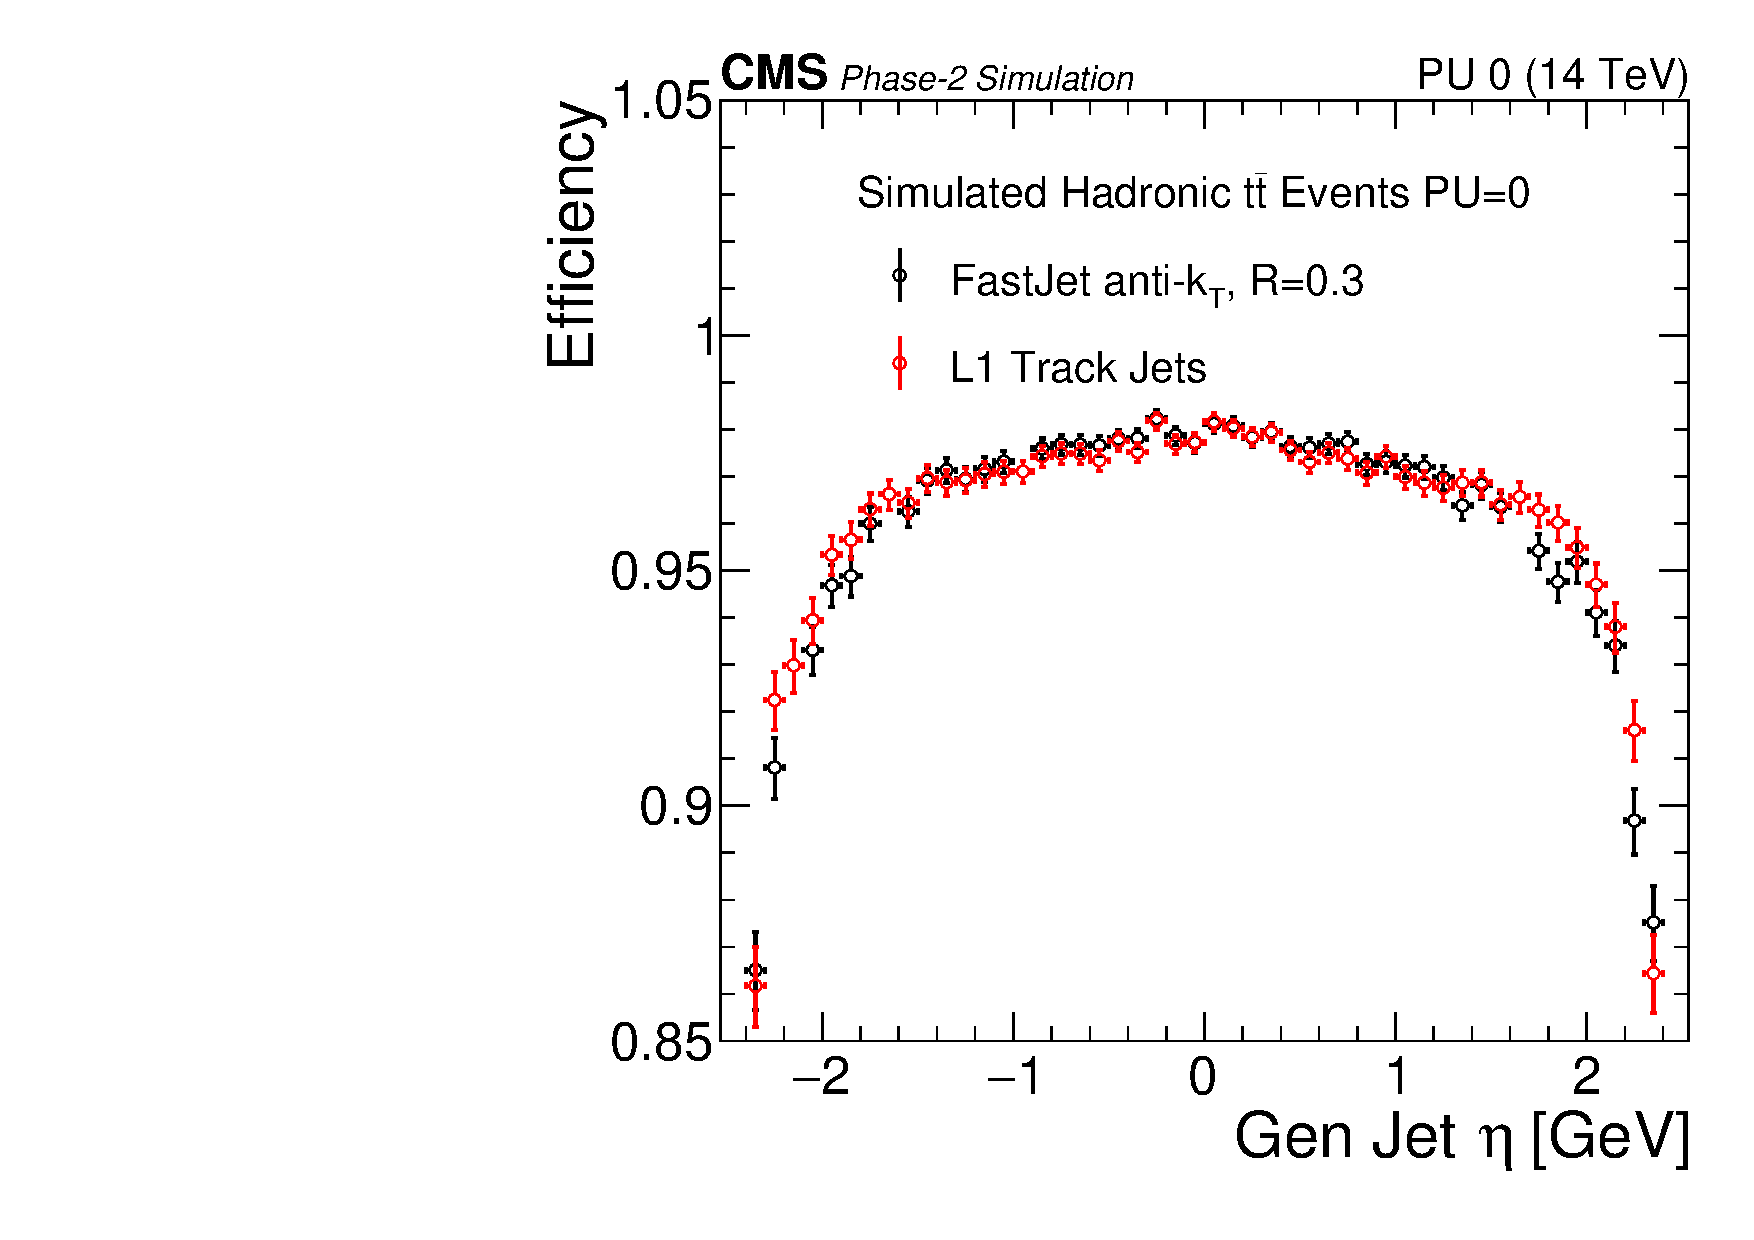
\includegraphics[width=0.45\textwidth ]{NoPUTTBarEff.pdf}
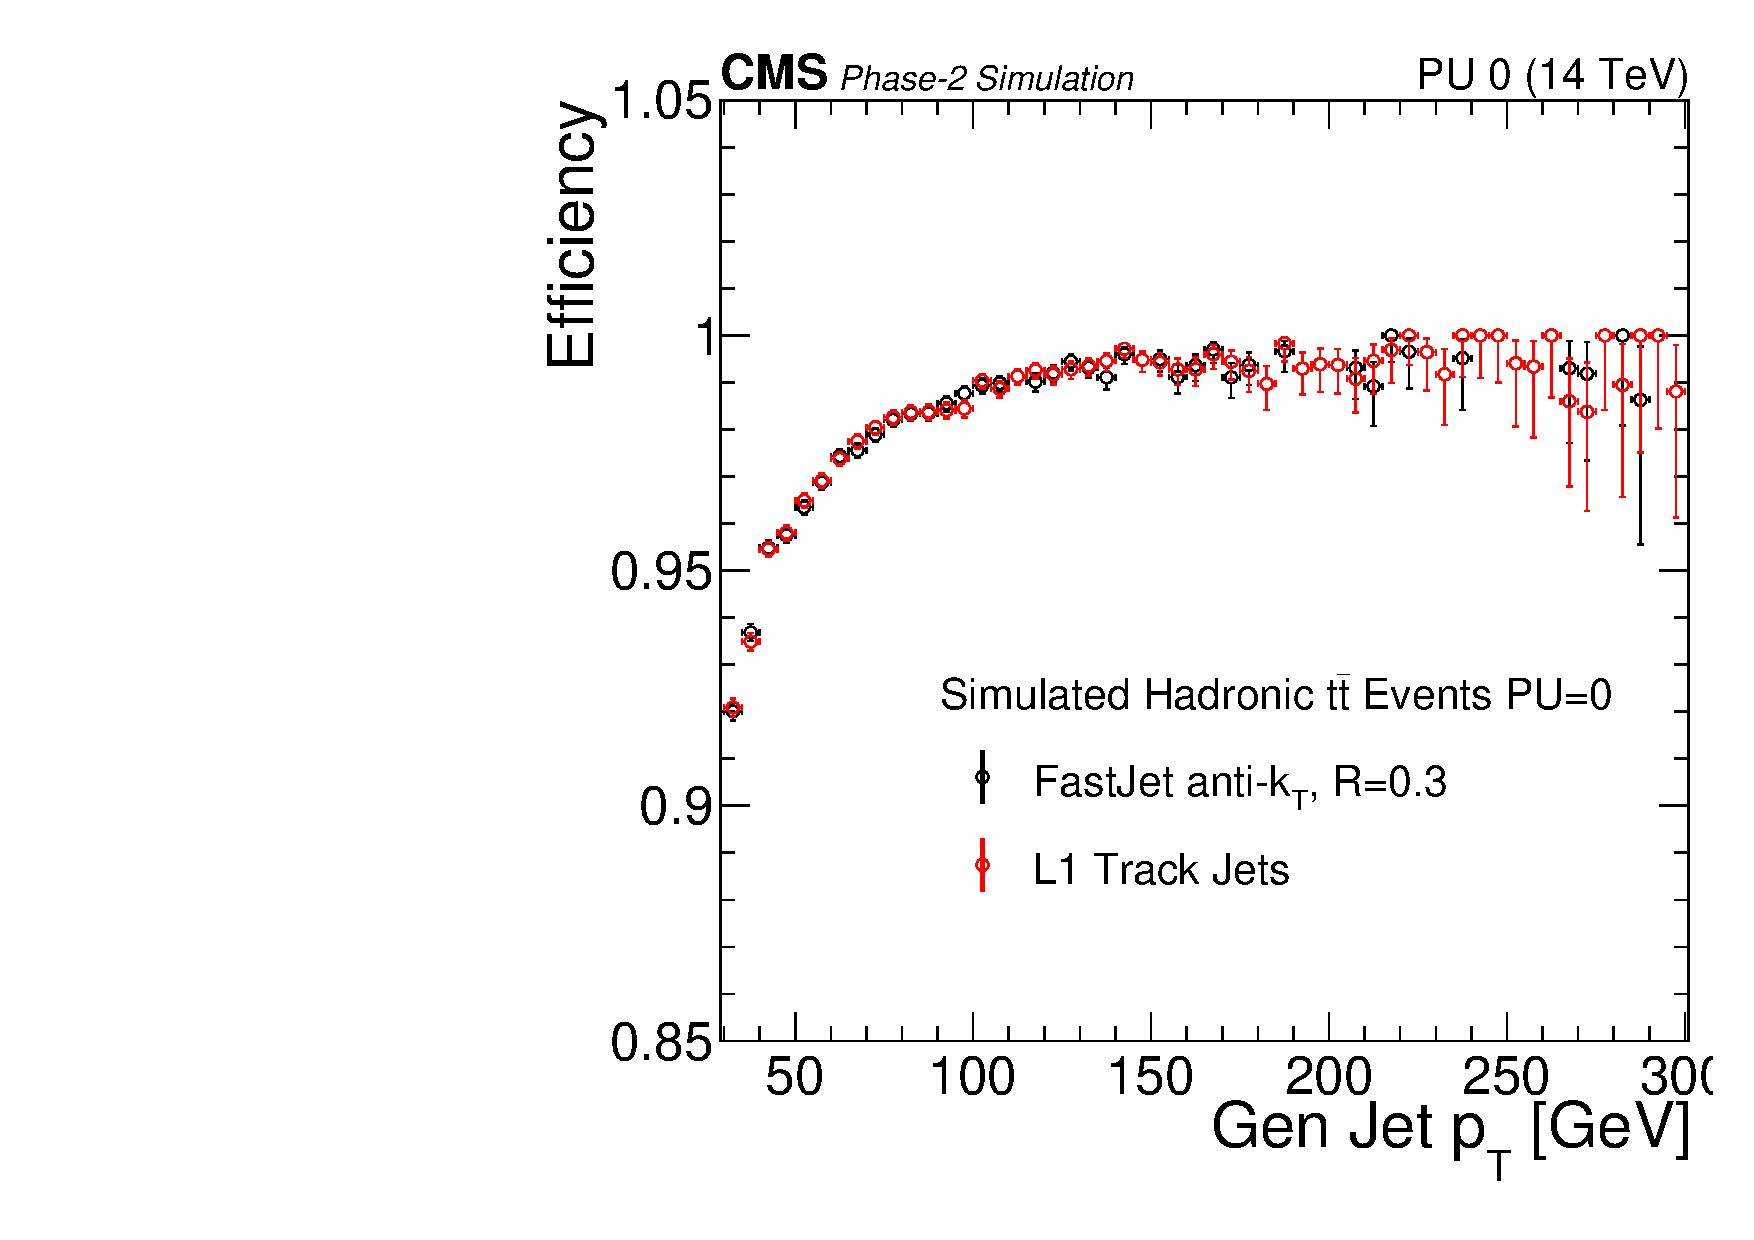
\includegraphics[width=0.45\textwidth]{NoPUTTBarPtEff.pdf}\\
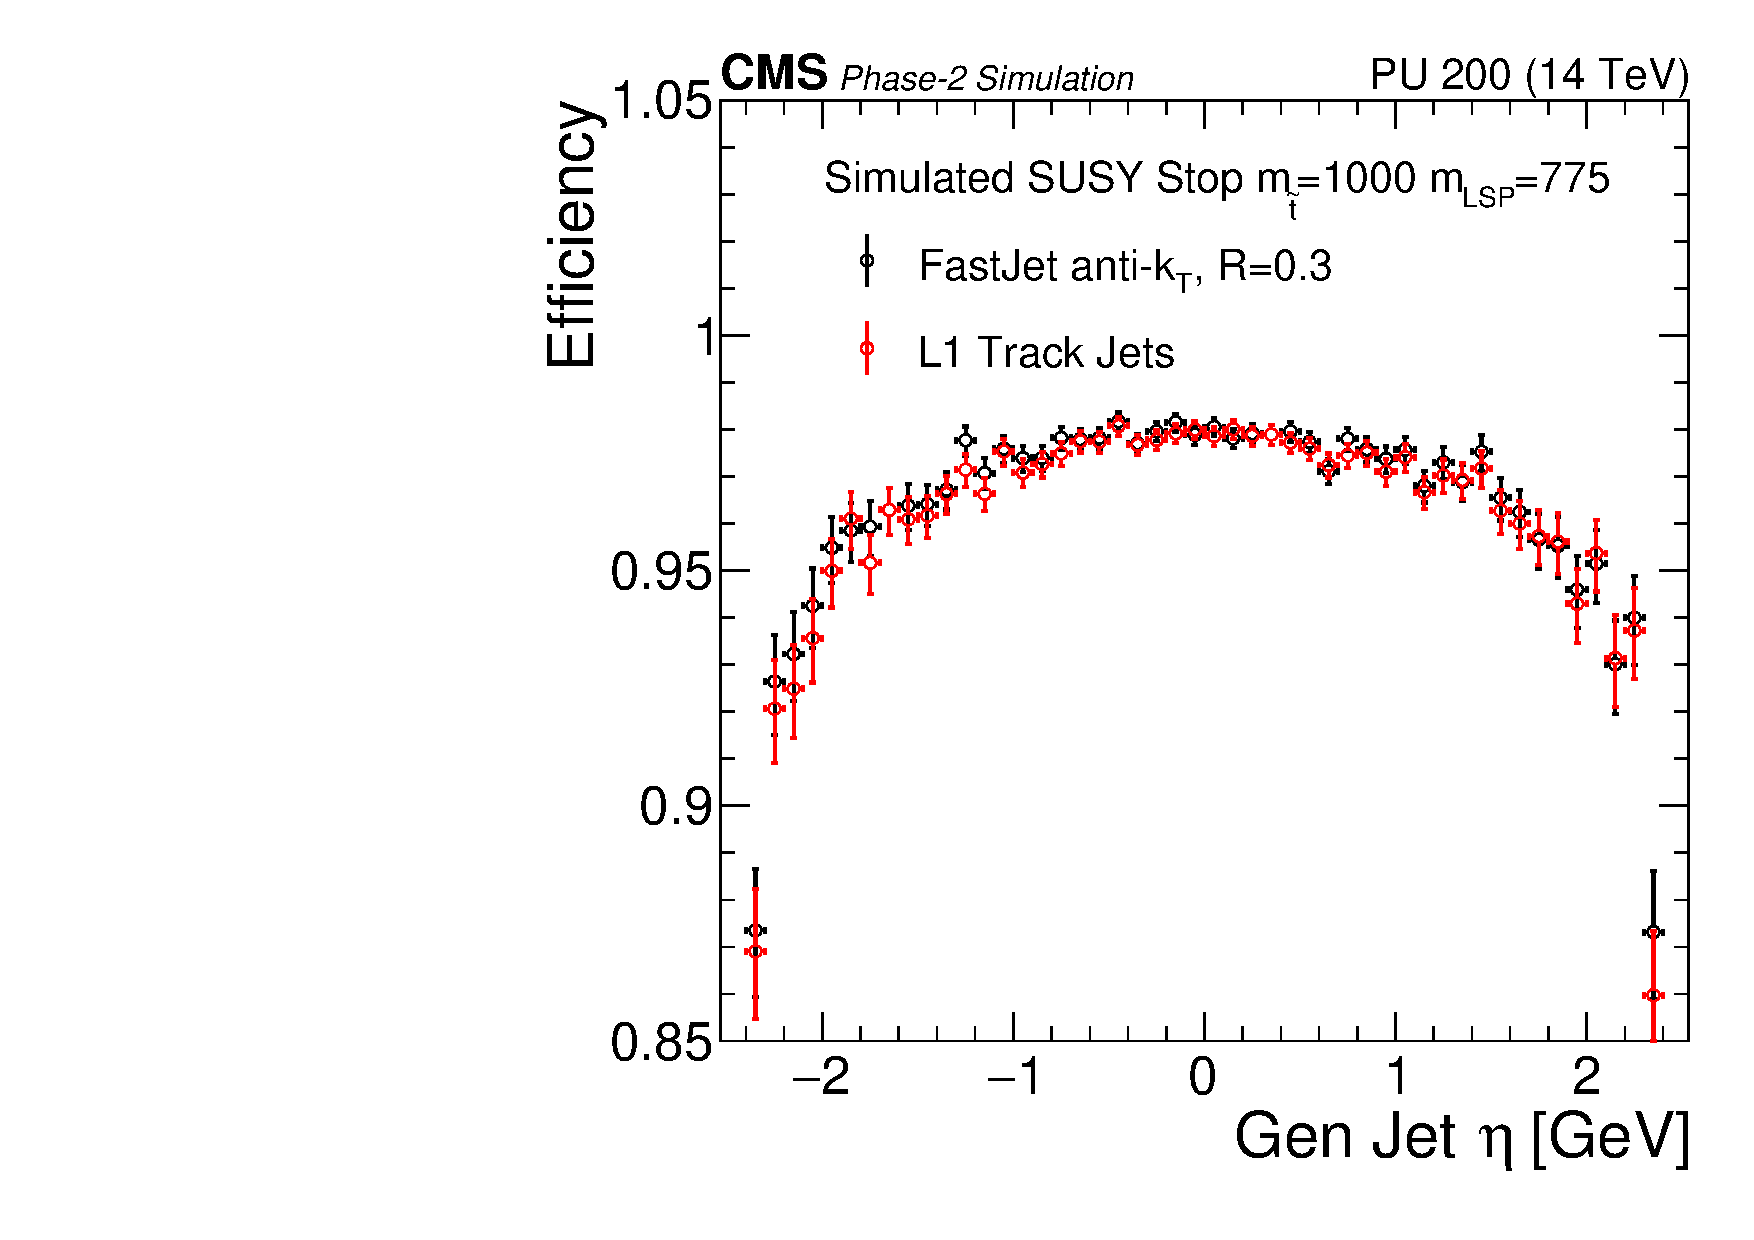
\includegraphics[width=0.45\textwidth]{StopSamplePUEtaEff.pdf}
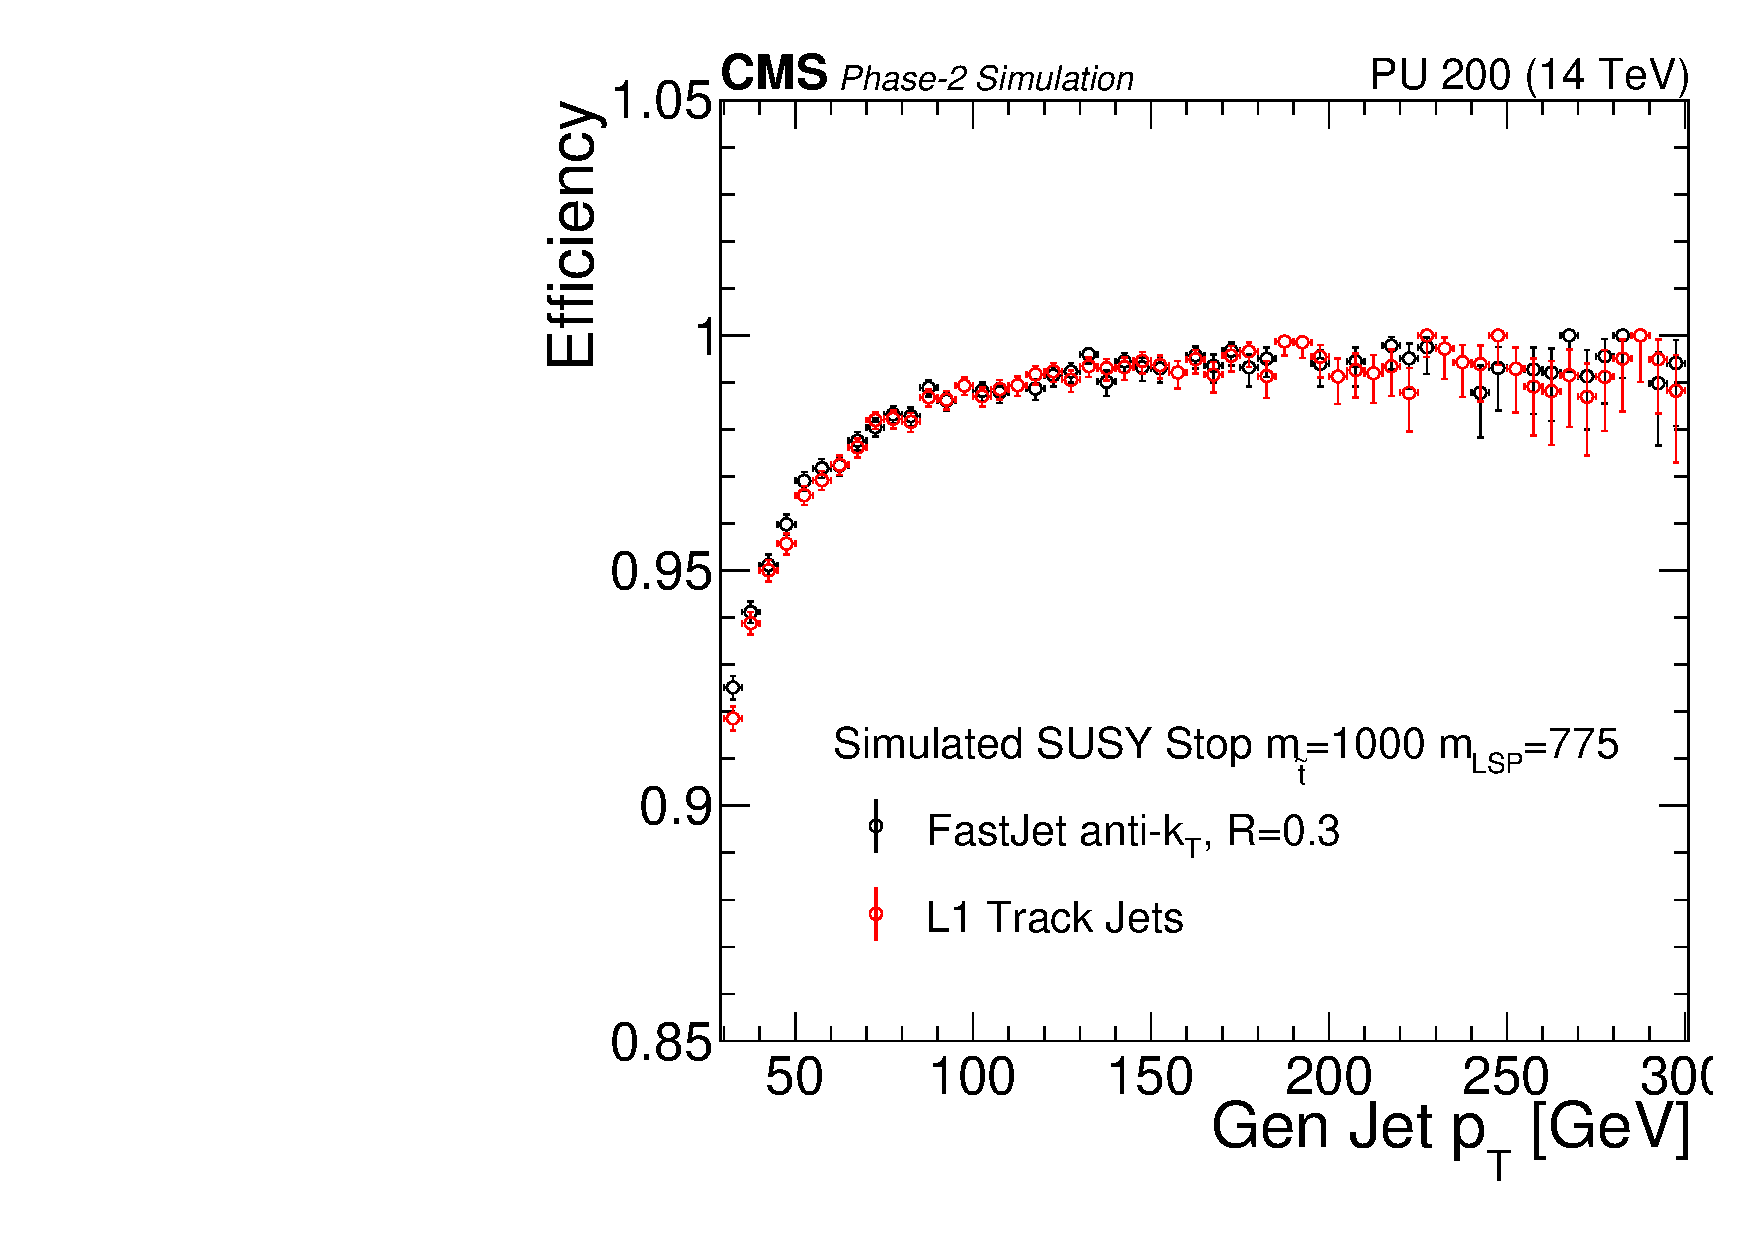
\includegraphics[width=0.45\textwidth]{StopSamplePUPtEff.pdf}
\caption{Comparison of the L1 track jet clustering and anti-$k_{T}$ clustering using FASTJET with $R=0.3$ with the same input collection of L1 reconstructed tracks. (top) The efficiency in fully hadronic t$\overline{t}$ with no pileup events as a function of generator $\eta$(left) and $p_{T}$ (right). The efficiency is computed by matching the generator-level jet to the reconstructed track jet within $\Delta R<0.4$. }
\label{fig:TkJetEfficiency}
\end{figure}

To keep global variables like L1 track-based $H_{T}$ and $H^{miss}_{T}$ resilient against pileup, we optimize the quality criteria on input L1 tracks to preserve a low trigger threshold while mantaining low data-taking rates. The same criteria as applied for track-based MET is used as in Table~\ref{tab:trkpurity}. When clustering tracks, the track multiplicity in each jet adds an additional handle to reject tracks from bad combinations of track hits which result in fake high $p_{T}$ tracks. In addition to the input track criteria, jets with $p_{T}>50$ are required to have at least 2 tracks and for $p_{T}>100$ are required to have at least 3 tracks. Track-based $H_{T}$  is computed as the scalar sum of $p_{T}$ for track jets with $p_{T}>5$GeV and the 4-vector of the same collection of jets is summed to compute $H^{miss}_{T}$. 

Figure~\ref{fig:TkPurityImprov} shows the improvement in both the L1 rate and signal efficiency for the L1 track-based $H_{T}$ and $H^{miss}_{T}$ along with the turn-on curves for a BSM stop signal point. The signal model simulates a supersymmetric top decay to its super-partner the top quark and stable lightest supersymmetric particle, $\tilde{\chi}^{1}_{0}$. The mass difference between the stop and $\tilde{\chi}^{1}_{0}$ is near the top-quark mass so that the missing transverse energy is still small. To measure the trigger turn on a collection of generator level jets is used to emulate offline  $H_{T}$ and $H^{miss}_{T}$ variables. The generator level collection of jets is made by clustering generator level particles, excluding neutrinos, using the anti-$k_{T}$ algorithm. The generator level jets considered are those with Gen Jet $p_{T}>30$GeV and $\vert\eta\vert<2.4$. 

As described in Section~\ref{sec:TkMET}, the rate decreases significantly for missing transverse momentum allowing to trigger on BSM signal events with moderate MET like this BSM stop model. Figure~\ref{fig:TkPurityImprov} shows the improvement in the L1 data-taking rate, the signal efficiency and the L1 turn-on when reducing the effect of tracks from bad track hit combinations. The improvement is seen for both the he L1 track-based $H_{T}$ and  $H^{miss}_{T}$ triggers. For a fixed L1 track-based $H_{T}$rate of 25 kHz, the $95\%$ off-line efficiency turn-on for the stop signal is lowered from 675GeV to 500GeV. The track-based $H^{miss}_{T}$  trigger lower the threshold from 675GeV down to 310GeV. In both cases, the signal efficiency is greatly increased for a fixed rate to trigger on the BSM stop phase-space with the track purity criteria.

\begin{figure}[htbp!]
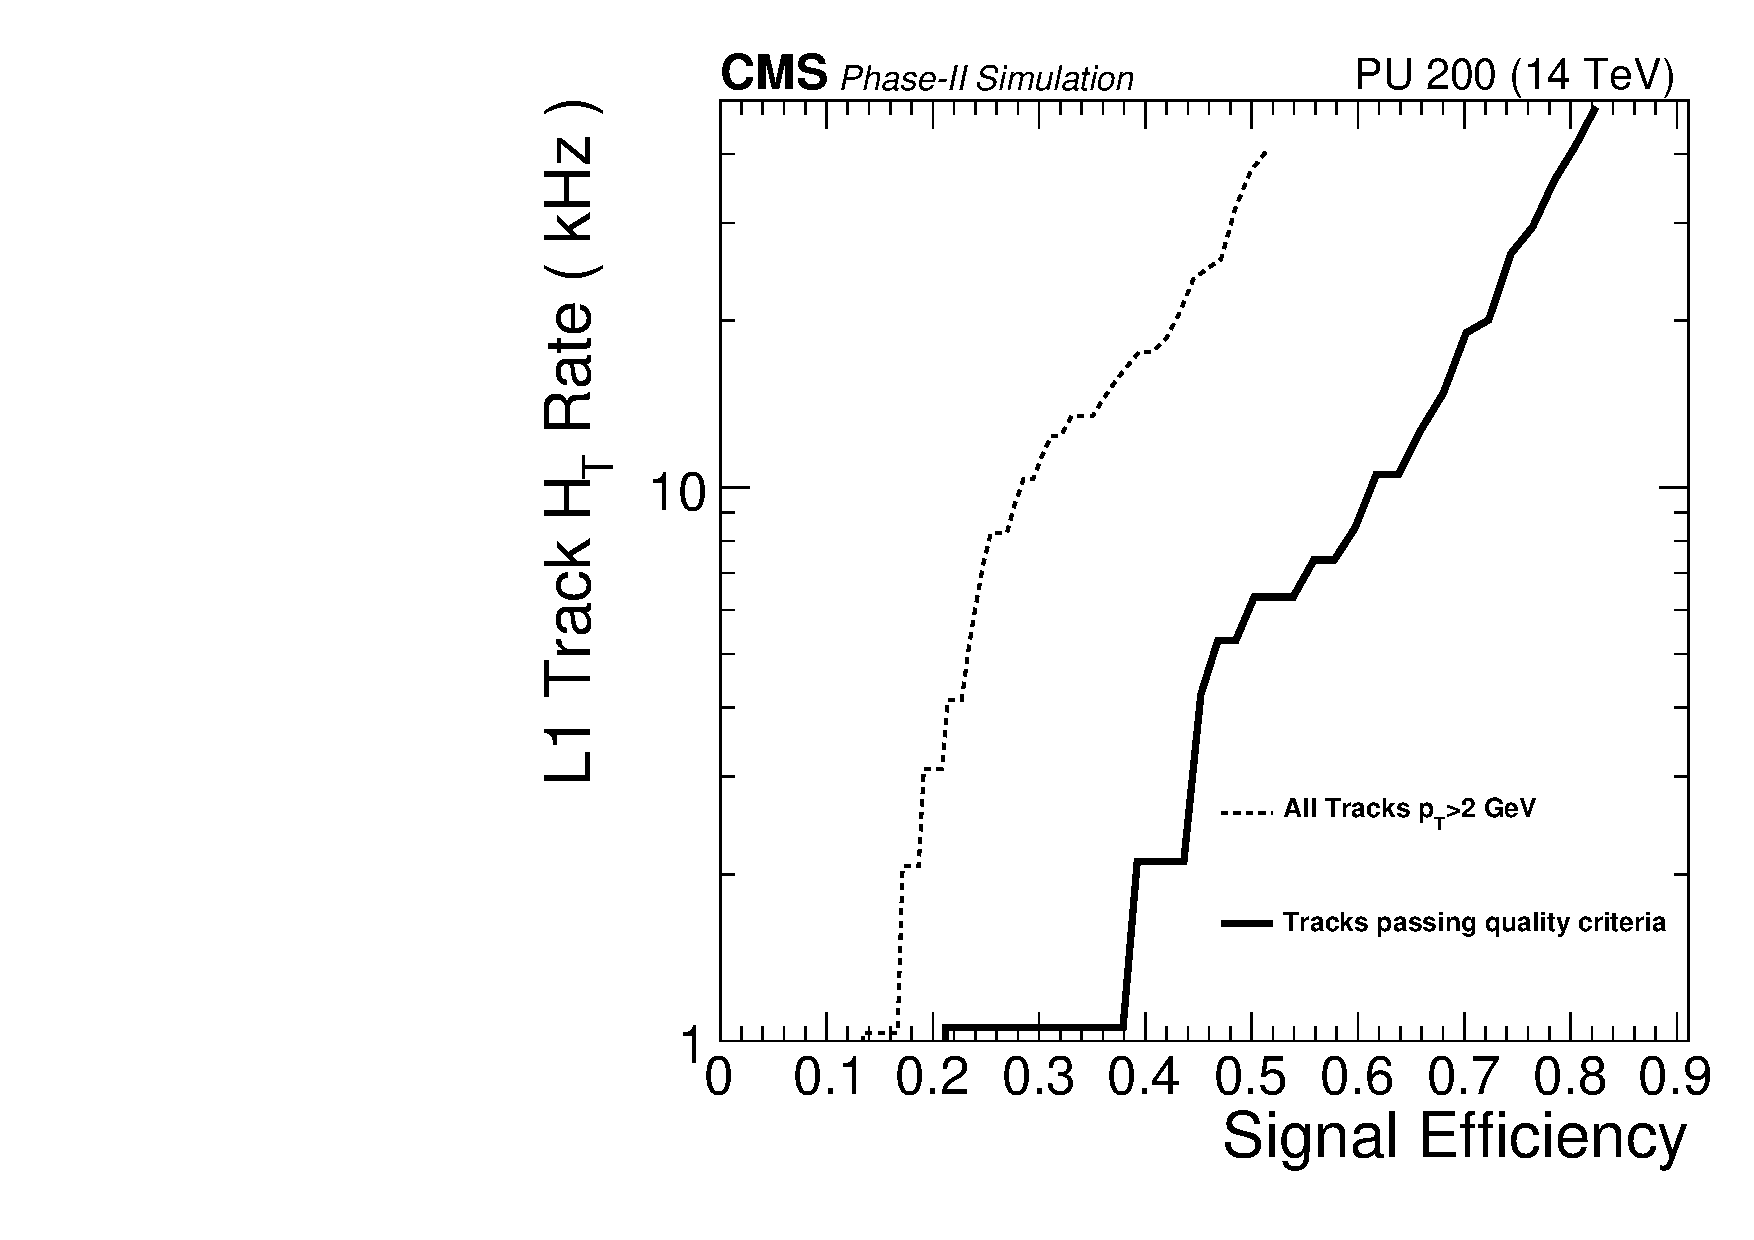
\includegraphics[width=0.45\textwidth ]{SignalEfficiencyVsRate_TkHT.pdf}
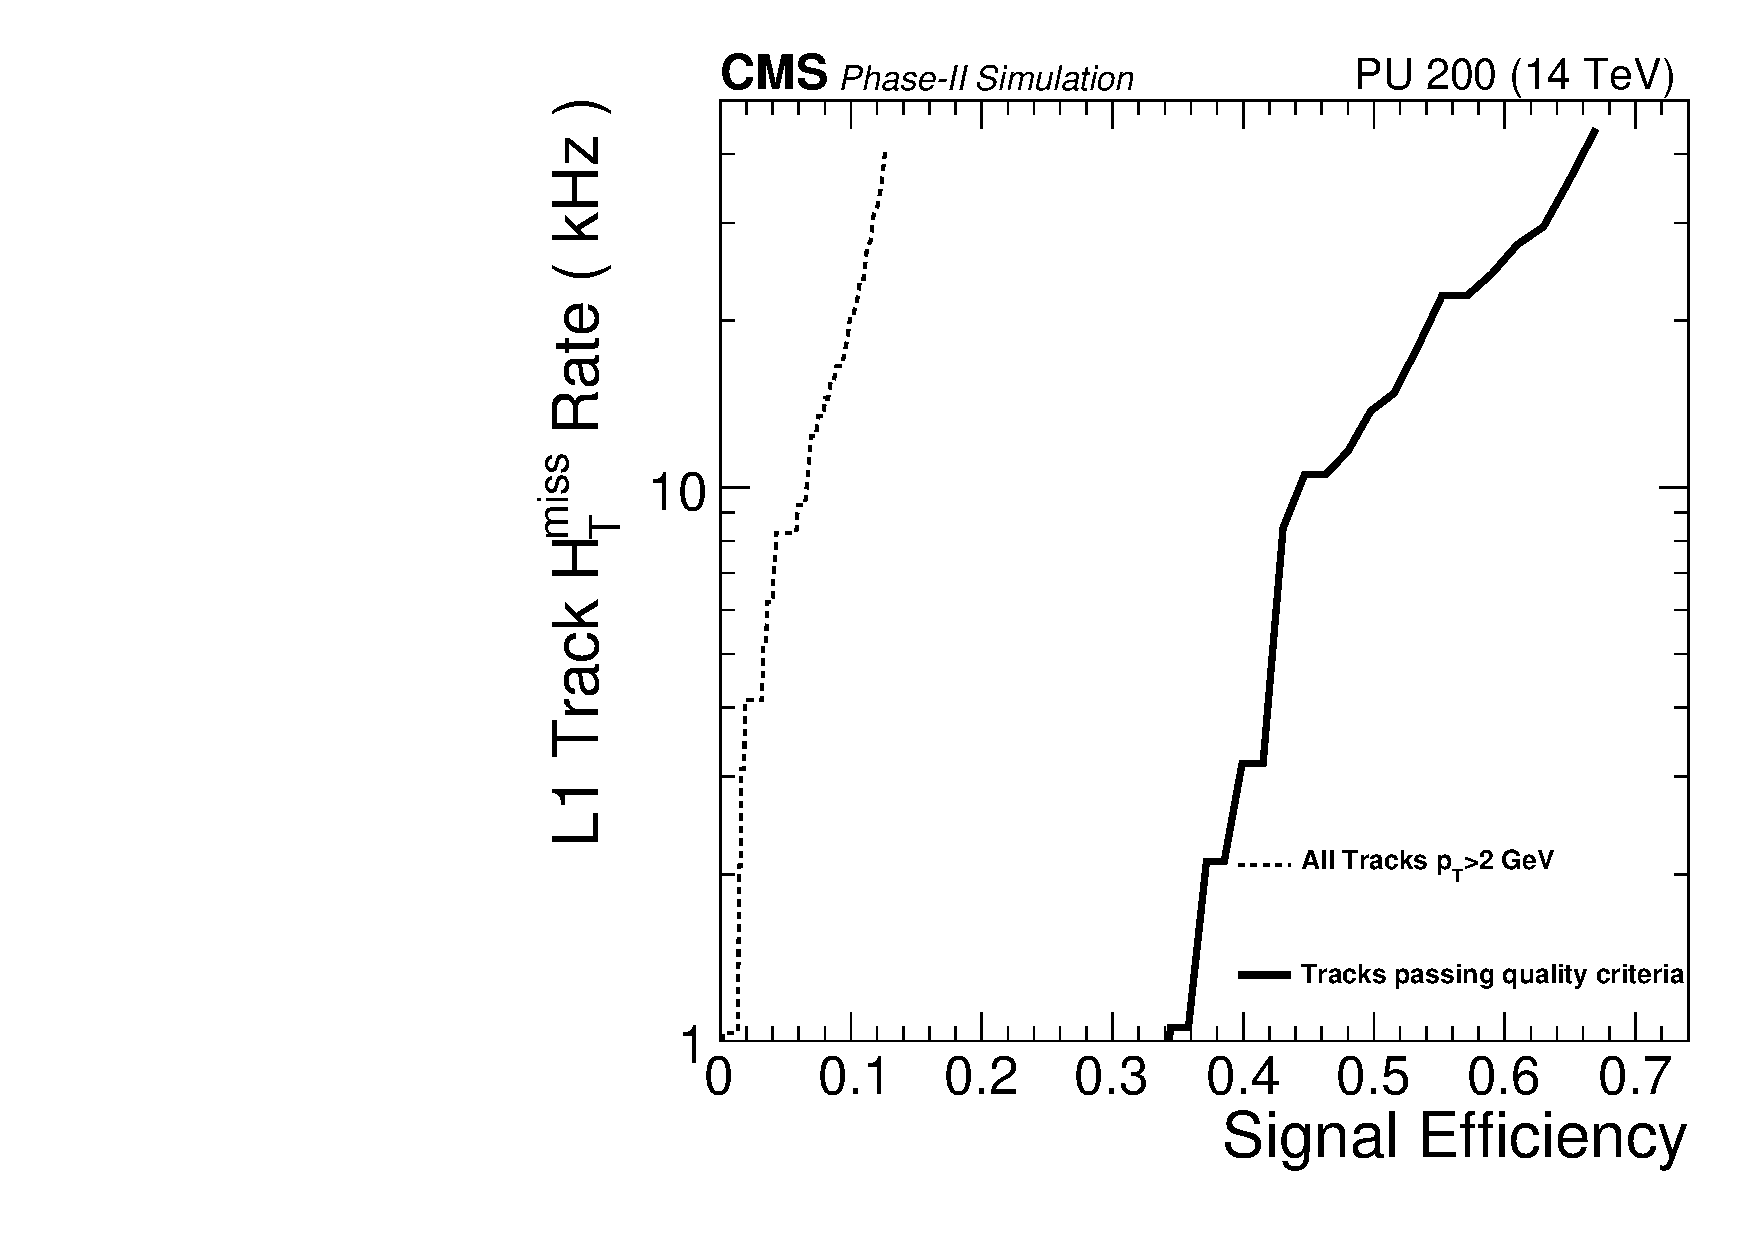
\includegraphics[width=0.45\textwidth ]{SignalEfficiencyVsRate_TkMHT.pdf}\\
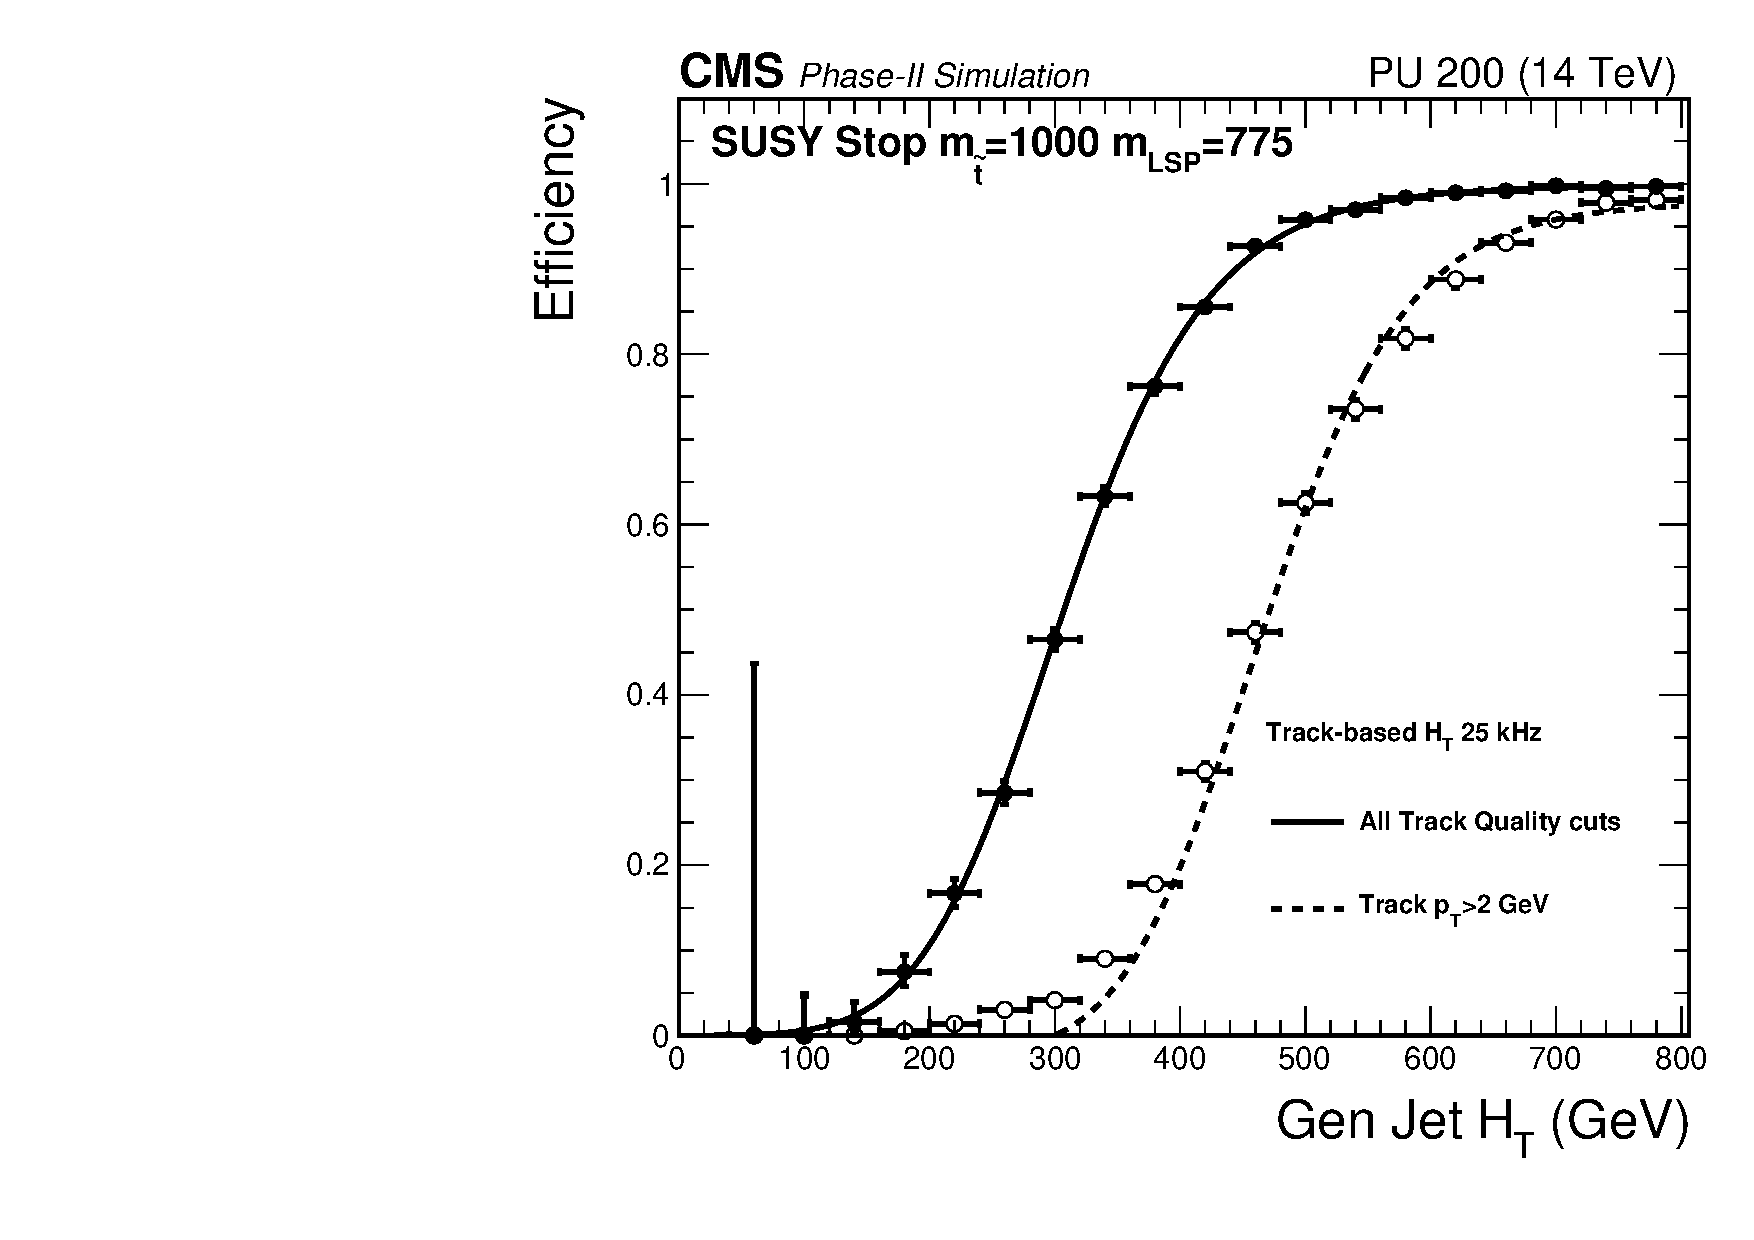
\includegraphics[width=0.45\textwidth ]{TurnOnTrackHT.pdf}
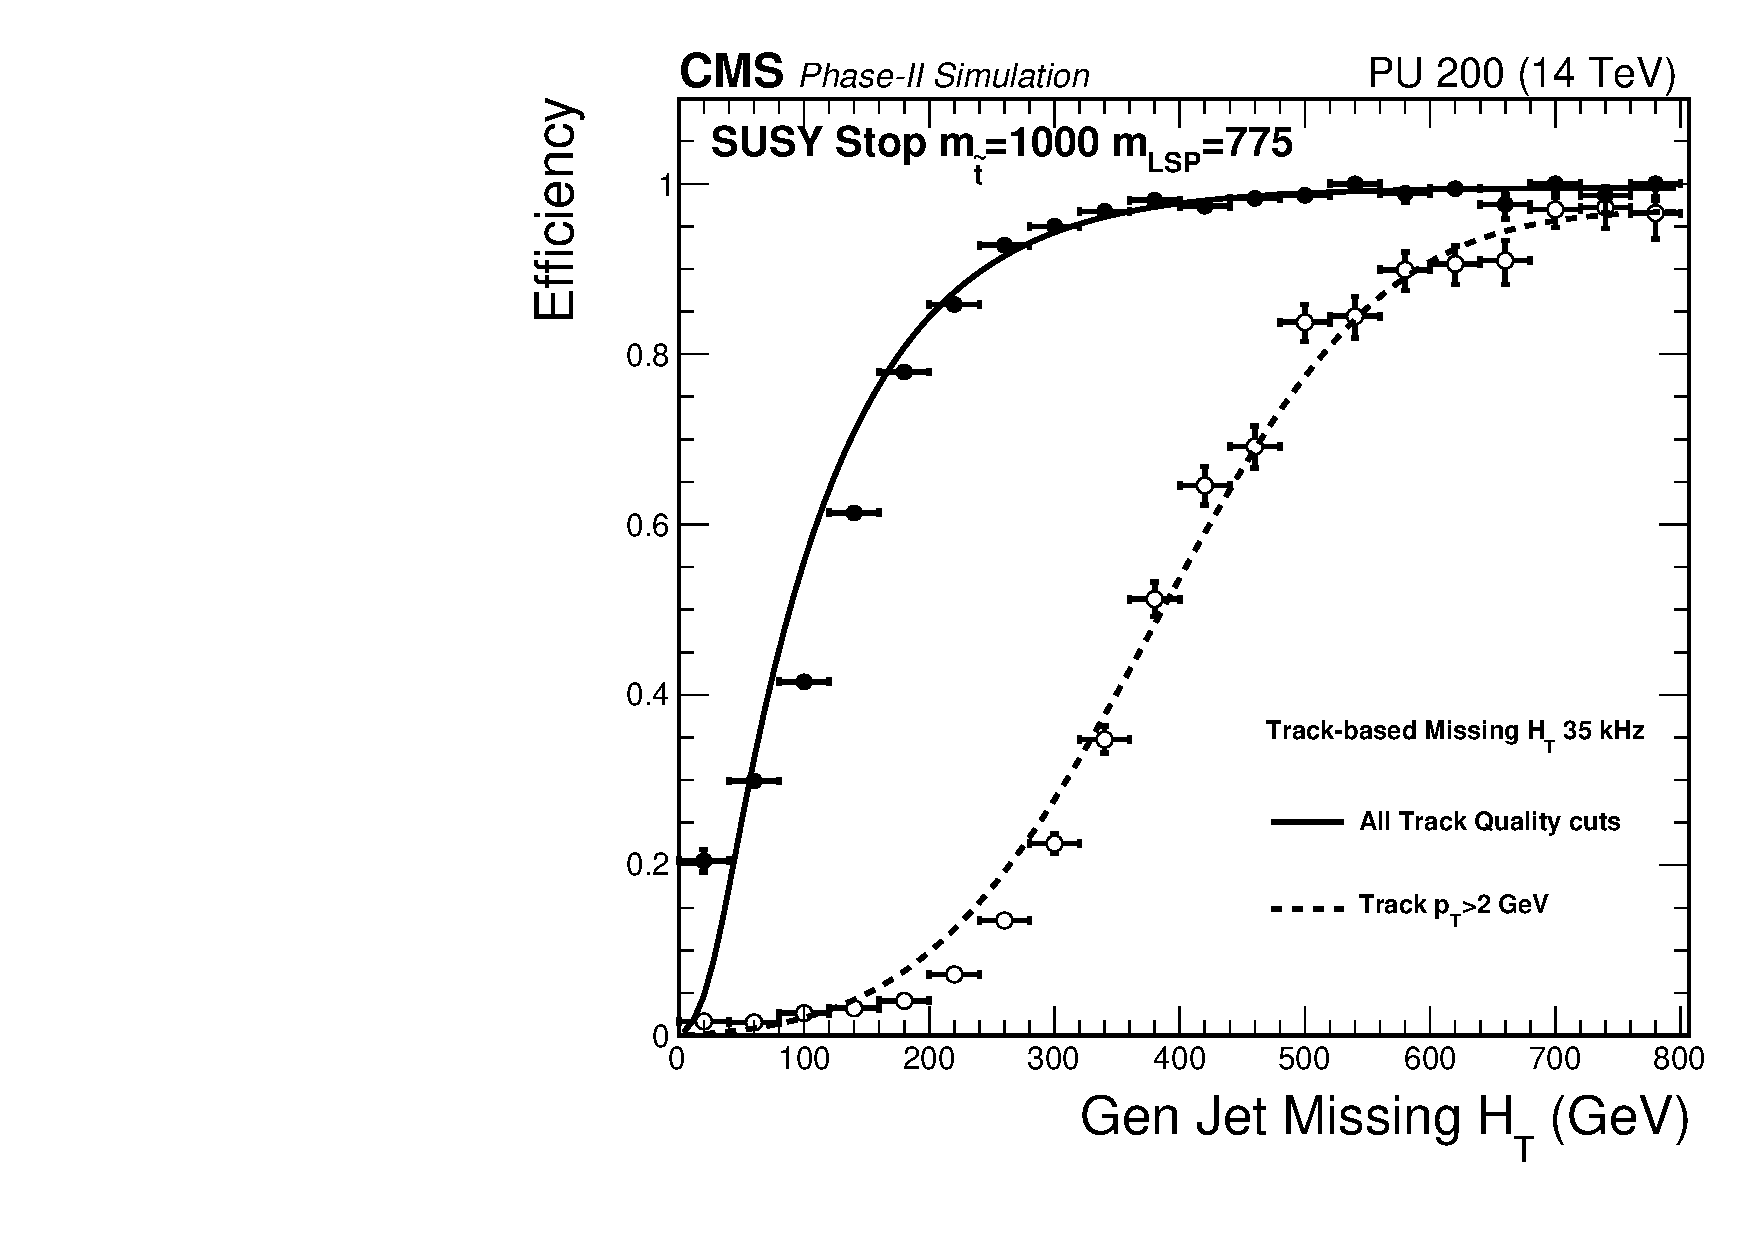
\includegraphics[width=0.45\textwidth ]{TurnOnTrackMHT.pdf}

\caption{(top) Signal efficiency versus L1 data-taking rates for (left) Track $H_{T}$ and (right) track $H^{miss}_{T}$. The track quality cuts allow to greatly lower these L1 thresholds for a fixed rate by rejecting fake high $p_{T}$ tracks. (bottom) The trigger-turn on efficiency based on generator level jets to emulate offline selection for the 25kHz L1 threshold for Track $H_{T}$(left) and 35kHz L1 threshold for $H^{miss}_{T}$(right). The efficiency turn-on for the BSM Stop signal at $95\%$ is greatly lowered with the track purity requirements.}
\label{fig:TkPurityImprov}
\end{figure}

%This section outlines a firmware implemented track clustering algorithm which takes as input a collection of tracks and outputs a collection of track jets. The algorithm does not rely on an input L1 primary vertex position. Instead the clustering is performed in z-regions across the beam spot and flags the jets from the primary collision based on the z-region with the largest track $H_{T}$. 

%The clustering in the $\eta$-$\phi$ plane is done in two 1-Dimensional steps. The first phase of the algorithm parses tracks into 27 $phi$ regions and 24 $\eta$ regions. Tracks are also required to pass the track purity requirements as for the track-based 